\documentclass[letterpaper]{article}
\usepackage[margin=1in]{geometry}
\usepackage[utf8]{inputenc}
\usepackage{textcomp}
\usepackage{amssymb}
\usepackage{natbib}
\usepackage{graphicx}
\usepackage{gensymb}
\usepackage{amsthm, amsmath, mathtools}
\usepackage[dvipsnames]{xcolor}
\usepackage{enumerate}
\usepackage{mdframed}
\usepackage[most]{tcolorbox}
\usepackage{csquotes}
% https://tex.stackexchange.com/questions/13506/how-to-continue-the-framed-text-box-on-multiple-pages

\tcbuselibrary{theorems}

\newcommand{\R}{\mathbb{R}}
\newcommand{\Z}{\mathbb{Z}}
\newcommand{\N}{\mathbb{N}}
\newcommand{\Q}{\mathbb{Q}}
\newcommand{\C}{\mathbb{C}}
\newcommand{\code}[1]{\texttt{#1}}
\newcommand{\mdiamond}{$\diamondsuit$}
\newcommand{\PowerSet}{\mathcal{P}}
\newcommand{\Mod}[1]{\ (\mathrm{mod}\ #1)}
\DeclareMathOperator{\lcm}{lcm}

%\newtheorem*{theorem}{Theorem}
%\newtheorem*{definition}{Definition}
%\newtheorem*{corollary}{Corollary}
%\newtheorem*{lemma}{Lemma}
\newtheorem*{proposition}{Proposition}


\newtcbtheorem[number within=section]{theorem}{Theorem}
{colback=green!5,colframe=green!35!black,fonttitle=\bfseries}{th}

\newtcbtheorem[number within=section]{definition}{Definition}
{colback=blue!5,colframe=blue!35!black,fonttitle=\bfseries}{def}

\newtcbtheorem[number within=section]{corollary}{Corollary}
{colback=yellow!5,colframe=yellow!35!black,fonttitle=\bfseries}{cor}

\newtcbtheorem[number within=section]{lemma}{Lemma}
{colback=red!5,colframe=red!35!black,fonttitle=\bfseries}{lem}

\newtcbtheorem[number within=section]{example}{Example}
{colback=white!5,colframe=white!35!black,fonttitle=\bfseries}{def}

\newtcbtheorem[number within=section]{note}{Important Note}{
        enhanced,
        sharp corners,
        attach boxed title to top left={
            xshift=-1mm,
            yshift=-5mm,
            yshifttext=-1mm
        },
        top=1.5em,
        colback=white,
        colframe=black,
        fonttitle=\bfseries,
        boxed title style={
            sharp corners,
            size=small,
            colback=red!75!black,
            colframe=red!75!black,
        } 
    }{impnote}
\usepackage[utf8]{inputenc}
\usepackage[english]{babel}
\usepackage{fancyhdr}
\usepackage[hidelinks]{hyperref}

\pagestyle{fancy}
\fancyhf{}
\rhead{MATH 155A}
\chead{Tuesday, April 12, 2022}
\lhead{Lecture 5}
\rfoot{\thepage}

\setlength{\parindent}{0pt}

\begin{document}

\section{Moving to \texorpdfstring{$\R^3$}{Three-Dimensions}}
For the most part, most of what we talked about in $\R^2$ applies here as well.

\subsection{The Basics}
We first begin by talking about some of the basics in $\R^3$. 

\subsubsection{Basic Notation in \texorpdfstring{$\R^3$}{Three-Dimensions}}
\begin{itemize}
    \item \textbf{Points:} In $\R^3$, points are triples. They are still written in vector form like so: 
    \[\mathbf{x} = \cyclic{x_1, x_2, x_3} = \begin{bmatrix}
        x_1 \\ x_2 \\ x_3
    \end{bmatrix}.\]

    \item \textbf{Axes:} In $\R^3$, the $xyz$-axes are in a different orientation than expected. In many other classes, $y$ is facing towards us; \underline{however}, in this course, $y$ will be facing upwards while $z$ is facing towards us. 
    \begin{center}
        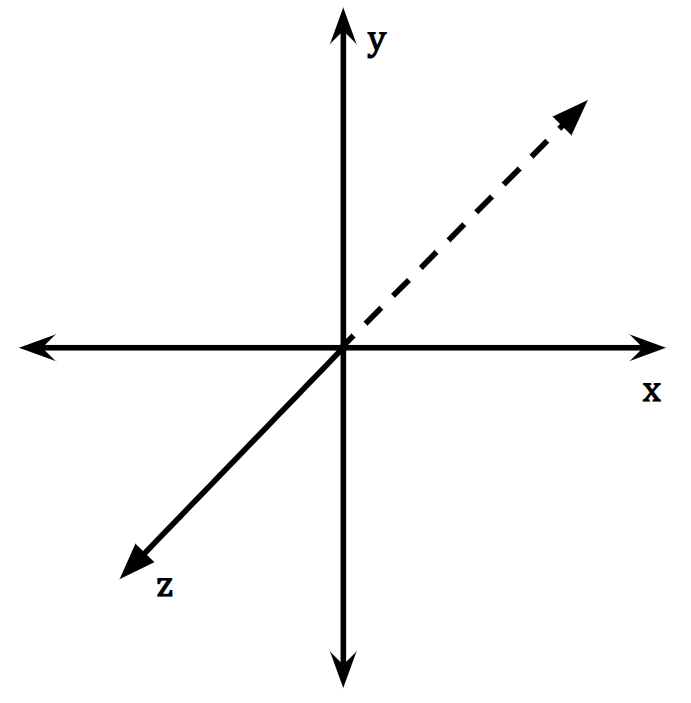
\includegraphics[scale=0.4]{../assets/axes3d.png}
    \end{center}
    As a side note, this is \emph{still} a right-handed coordinate system. The cross product rule still uses the right-hand rule. 

    \item \textbf{Standard Basis Vectors:} The standard basis vectors (unit vectors) in $\R^3$ are as follows: 
    \[\mathbf{i} = \begin{bmatrix}
        1 \\ 0 \\ 0
    \end{bmatrix} \qquad \mathbf{j} = \begin{bmatrix}
        0 \\ 1 \\ 0
    \end{bmatrix} \qquad \mathbf{k} = \begin{bmatrix}
        0 \\ 0 \\ 1
    \end{bmatrix}.\]
\end{itemize}

\subsubsection{Transformations}
In particular, linear transformations, translations, and affine transformations are \textbf{identical} to the definitions on $\R^2$. To see what we mean, consider the following:
\begin{itemize}
    \item \textbf{Translations:} A translation is defined by 
    \[T_{\mathbf{u}}(\mathbf{x}) = \mathbf{x} + \mathbf{u},\]
    where $\mathbf{u} = \begin{bmatrix}
        u_1 \\ u_2 \\ u_3
    \end{bmatrix} \in \R^3$. 

    \item \textbf{Affine Transformation:} An affine transformation is defined by 
    \[A(\mathbf{x}) = B(\mathbf{x}) + \mathbf{u},\]
    where $B$ is linear. 
\end{itemize}
Consider the following \emph{scaling} transformations: 
\begin{itemize}
    \item \textbf{Uniform Scaling:} For some $\alpha \in \R$, uniform scaling just scales the vector $\mathbf{x}$ by a factor of $\alpha$. So, we have 
    \[S_{\alpha}(\mathbf{x}) = \alpha \mathbf{x}.\]

    \item \textbf{General Scaling:} For some $\alpha, \beta, \gamma \in \R$, scaling a vector involves multiplying each of the constant terms by the corresponding terms in the vector. That is, 
    \[S_{\cyclic{\alpha, \beta, \gamma}}\left(\begin{bmatrix}
        x_1 \\ x_2 \\ x_3
    \end{bmatrix}\right) = \begin{bmatrix}
        \alpha x_1 \\ 
        \beta x_2 \\ 
        \gamma x_3
    \end{bmatrix}.\]
\end{itemize}

\subsubsection{Rotations Around the Origin}
Rotations in $\R^3$ are more complicated. Here, we denote $R_{\theta, \mathbf{u}}$ to be the rotation angle $\theta$ around axis $\mathbf{u}$, where $\mathbf{u} \neq \mathbf{0}$. The direction is given by the right-hand rule. 

\begin{mdframed}[]
    (Example.) Consider $R_{\frac{\pi}{2}, \mathbf{i}}$, which is a 90 degree rotation (or $\pi / 2$ radians) around the $x$-axis. How does $R_{\frac{\pi}{2}, \mathbf{i}}$ act on the standard basis vectors $\mathbf{i}$, $\mathbf{j}$, and $\mathbf{k}$?

    \begin{mdframed}[]
        First, we're holding the $x$-axis fixed since we're rotating around the $x$-axis. Thus, this rotation will map $\mathbf{i}$ to itself. Next, we note that $\mathbf{j}$ will be mapped to $\mathbf{k}$. Likewise, $\mathbf{k}$ will be mapped to $-\mathbf{j}$.
    \end{mdframed}
\end{mdframed}

\subsubsection{Matrix Representation of Linear Transformations}
Now, we'll talk about $3 \times 3$ matrix representations of linear transformations. These are more or less the same thing as in $\R^2$. 

\begin{mdframed}[]
    (Example.) $S_{\cyclic{\alpha, \beta, \gamma}}$ is represented by 
    \[\begin{bmatrix}
        \alpha & 0 & 0 \\ 
        0 & \beta & 0 \\ 
        0 & 0 & \gamma
    \end{bmatrix}.\]
\end{mdframed}

\begin{mdframed}[]
    (Example.) Consider $R_{\frac{\pi}{2}, \mathbf{k}}$, which is a 90 degree rotation around the $z$-axis. We note that: 
    \begin{itemize}
        \item The $\mathbf{i}$ vector is mapped to the $\mathbf{j}$ vector.
        \item The $\mathbf{j}$ vector is mapped to the $-\mathbf{i}$ vector. 
        \item The $\mathbf{k}$ vector is mapped to itself. 
    \end{itemize}
    Therefore, the matrix representation of this rotation is given by 
    \[\begin{bmatrix}
        0 & -1 & 0 \\ 
        1 & 0 & 0 \\ 
        0 & 0 & 1
    \end{bmatrix}.\]
\end{mdframed}
More generally, if $A$ is a linear transformation, we let $\mathbf{u} = A(\mathbf{i})$, $\mathbf{v} = A(\mathbf{j})$, and $\mathbf{w} = A(\mathbf{k})$. Then, $A$ is represented by the $3 \times 3$ matrix 
\[M = \begin{bmatrix}
    \mathbf{u} & \mathbf{v} & \mathbf{w}
\end{bmatrix} = \begin{bmatrix}
    u_1 & v_1 & w_1 \\ 
    u_2 & v_2 & w_2 \\ 
    u_3 & v_3 & w_3 
\end{bmatrix}.\]

\subsubsection{Homogeneous Coordinates \& Matrix Representations of Affine Transformations}
We define the four-tuple $\cyclic{x, y, z, w}$ to be a \textbf{homogeneous} representation of $\cyclic{\frac{x}{w}, \frac{y}{w}, \frac{z}{w}} \in \R^3$, where $w \neq 0$.

\bigskip 

Let us now suppose that $A(\mathbf{x}) = B(\mathbf{x}) + \mathbf{t}$, where $B$ is a linear transformation and $\mathbf{t} = \begin{bmatrix}
    t_1 \\ t_2 \\ t_3
\end{bmatrix} \in \R^3$, so that $A$ is affine. Suppose that $B$ is a $3 \times 3$ matrix representation
\[M = \begin{bmatrix}
    m_{1,1} & m_{1,2} & m_{1,3} \\ 
    m_{2,1} & m_{2,2} & m_{2,3} \\ 
    m_{3,1} & m_{3,2} & m_{3,3} 
\end{bmatrix}.\]
Then, the $4 \times 4$ matrix 
\[N = \begin{bmatrix}
    M & \mathbf{t} \\ 
    \mathbf{0}^T & 1
\end{bmatrix} = \begin{bmatrix}
    m_{1,1} & m_{1,2} & m_{1,3} & t_1 \\ 
    m_{2,1} & m_{2,2} & m_{2,3} & t_2 \\ 
    m_{3,1} & m_{3,2} & m_{3,3} & t_3 \\ 
    0 & 0 & 0 & 1
\end{bmatrix}\]
represents the affine transformation $A$.


\subsection{Rigid \& Orientation-Preserving Transformations}
We first begin by talking about these in \emph{both} $\R^2$ and $\R^3$. 
\begin{definition}{Rigid}{}
    A transformation $A$ is \textbf{rigid} if the following conditions hold: 
    \begin{itemize}
        \item It preserves distances between points; that is, for all $\mathbf{x}, \mathbf{y} \in \R^2$ (or $\R^3$),
        \[||A(\mathbf{x}) - A(\mathbf{y})|| = ||\mathbf{x} - \mathbf{y}||.\]

        \item It preserves angles. To see what we mean here, if we have two vectors $\mathbf{u}$ and a vector $\mathbf{v}$, both rooted at some point, then suppose these two vectors form an angle $\theta$. Then, the idea is that $A(\mathbf{u})$ and $A(\mathbf{v})$ also has the same angle $\theta$.
    \end{itemize}
\end{definition}
\textbf{Remark:} We say that $||\mathbf{u}||$, the magnitude (also called \emph{norm} or \emph{length}), is equal to:
\begin{itemize}
    \item $\sqrt{u_1^2 + u_2^2}$ in $\R^2$ if $\mathbf{u} = \begin{bmatrix}
        u_1 \\ u_2
    \end{bmatrix}$. 
    \item $\sqrt{u_1^2 + u_2^2 + u_3^3}$ in $\R^3$ if $\mathbf{u} = \begin{bmatrix}
        u_1 \\ u_2 \\ u_3
    \end{bmatrix}$. 
\end{itemize}

\subsubsection{Orientation-Preserving in \texorpdfstring{$\R^2$}{Two-Dimensions}}
\begin{definition}{Orientation-Preserving in $\R^2$}{}
    In $\R^2$, an affine transformation $A$ is \textbf{orientation-preserving} if it preserves the direction of angles. 
\end{definition}
Consider the following figure, where $A$ is an orientation-preserving transformation and $B$ is not an orientation-preserving transformation (sometimes known as \emph{orientation-reversing}).
\begin{center}
    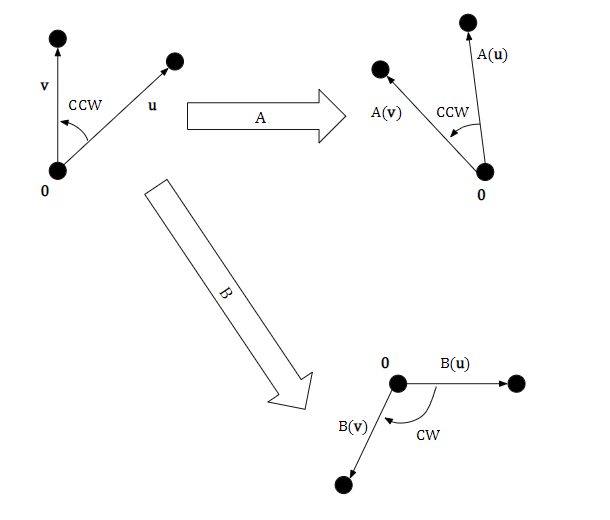
\includegraphics[scale=0.8]{../assets/orientation.png}
\end{center}
In particular, rotations are orientation-preserving whereas reflections are not orientation-preserving.

\subsubsection{Orientation-Preserving in \texorpdfstring{$\R^3$}{Three-Dimensions}}
Informally, in $\R^3$, an affine transformation $A$ is \textbf{orientation-preserving} if it preserves the ``right-hand'' rule.
\begin{theorem}{}{}
    Let $M$, a $3 \times 3$ matrix, represent the linear transformation $A$. Then, $A$ is orientation-preserving if and only if $\det(M) > 0$. 
\end{theorem}

\end{document}